% Created by tikzDevice version 0.12.6 on 2025-04-24 16:39:48
% !TEX encoding = UTF-8 Unicode
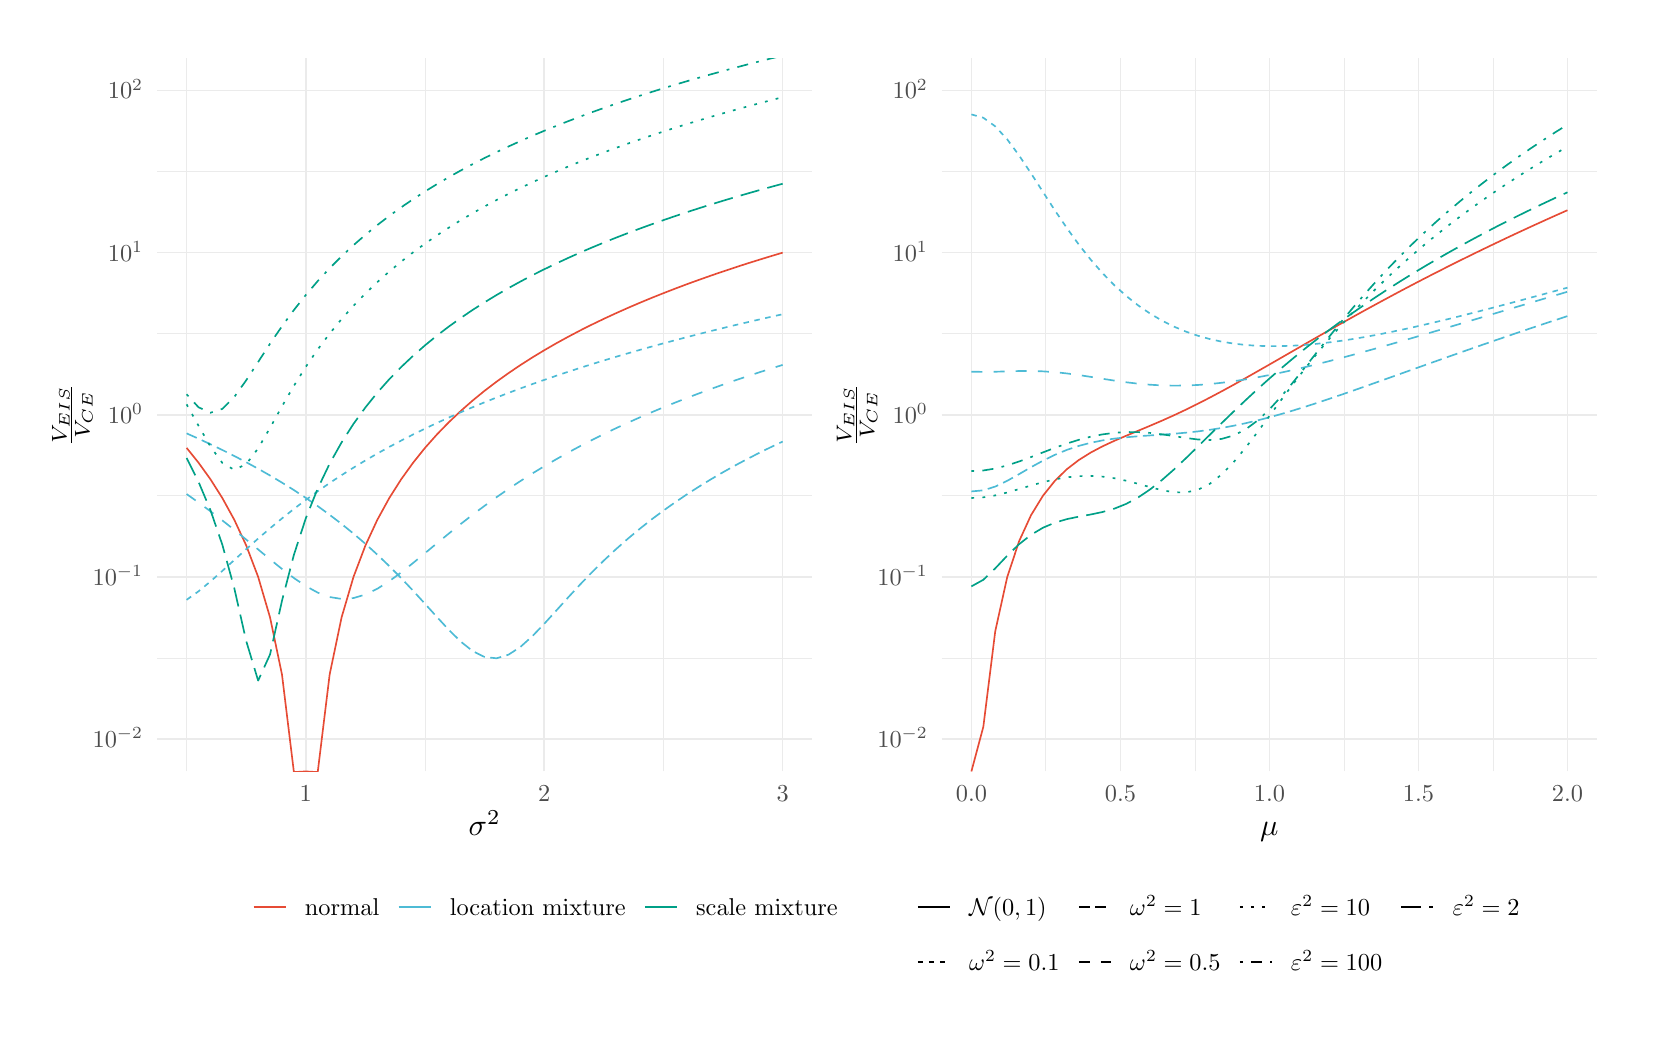
\begin{tikzpicture}[x=1pt,y=1pt]
\definecolor{fillColor}{RGB}{255,255,255}
\path[use as bounding box,fill=fillColor,fill opacity=0.00] (0,0) rectangle (578.16,361.35);
\begin{scope}
\path[clip] ( 46.66, 92.59) rectangle (283.58,350.35);
\definecolor{drawColor}{gray}{0.92}

\path[draw=drawColor,line width= 0.3pt,line join=round] ( 46.66,133.60) --
	(283.58,133.60);

\path[draw=drawColor,line width= 0.3pt,line join=round] ( 46.66,192.18) --
	(283.58,192.18);

\path[draw=drawColor,line width= 0.3pt,line join=round] ( 46.66,250.76) --
	(283.58,250.76);

\path[draw=drawColor,line width= 0.3pt,line join=round] ( 46.66,309.34) --
	(283.58,309.34);

\path[draw=drawColor,line width= 0.3pt,line join=round] ( 57.43, 92.59) --
	( 57.43,350.35);

\path[draw=drawColor,line width= 0.3pt,line join=round] (143.58, 92.59) --
	(143.58,350.35);

\path[draw=drawColor,line width= 0.3pt,line join=round] (229.74, 92.59) --
	(229.74,350.35);

\path[draw=drawColor,line width= 0.6pt,line join=round] ( 46.66,104.31) --
	(283.58,104.31);

\path[draw=drawColor,line width= 0.6pt,line join=round] ( 46.66,162.89) --
	(283.58,162.89);

\path[draw=drawColor,line width= 0.6pt,line join=round] ( 46.66,221.47) --
	(283.58,221.47);

\path[draw=drawColor,line width= 0.6pt,line join=round] ( 46.66,280.05) --
	(283.58,280.05);

\path[draw=drawColor,line width= 0.6pt,line join=round] ( 46.66,338.63) --
	(283.58,338.63);

\path[draw=drawColor,line width= 0.6pt,line join=round] (100.51, 92.59) --
	(100.51,350.35);

\path[draw=drawColor,line width= 0.6pt,line join=round] (186.66, 92.59) --
	(186.66,350.35);

\path[draw=drawColor,line width= 0.6pt,line join=round] (272.81, 92.59) --
	(272.81,350.35);
\definecolor{drawColor}{RGB}{230,75,53}

\path[draw=drawColor,line width= 0.6pt,line join=round] ( 57.43,209.51) --
	( 61.74,204.15) --
	( 66.05,198.16) --
	( 70.35,191.37) --
	( 74.66,183.52) --
	( 78.97,174.25) --
	( 83.28,162.89) --
	( 87.58,148.25) --
	( 91.89,127.62) --
	( 96.20, 92.35) --
	(100.51, 92.59) --
	(104.81, 92.35) --
	(109.12,127.62) --
	(113.43,148.25) --
	(117.74,162.89) --
	(122.05,174.25) --
	(126.35,183.52) --
	(130.66,191.37) --
	(134.97,198.16) --
	(139.28,204.15) --
	(143.58,209.51) --
	(147.89,214.36) --
	(152.20,218.79) --
	(156.51,222.86) --
	(160.81,226.63) --
	(165.12,230.15) --
	(169.43,233.43) --
	(173.74,236.51) --
	(178.04,239.42) --
	(182.35,242.17) --
	(186.66,244.78) --
	(190.97,247.27) --
	(195.27,249.63) --
	(199.58,251.90) --
	(203.89,254.06) --
	(208.20,256.14) --
	(212.50,258.13) --
	(216.81,260.05) --
	(221.12,261.90) --
	(225.43,263.69) --
	(229.74,265.41) --
	(234.04,267.08) --
	(238.35,268.70) --
	(242.66,270.26) --
	(246.97,271.78) --
	(251.27,273.26) --
	(255.58,274.69) --
	(259.89,276.09) --
	(264.20,277.44) --
	(268.50,278.76) --
	(272.81,280.05);
\definecolor{drawColor}{RGB}{77,187,213}

\path[draw=drawColor,line width= 0.6pt,dash pattern=on 2pt off 2pt ,line join=round] ( 57.43,154.60) --
	( 61.74,157.67) --
	( 66.05,161.24) --
	( 70.35,165.06) --
	( 74.66,168.99) --
	( 78.97,172.90) --
	( 83.28,176.74) --
	( 87.58,180.45) --
	( 91.89,184.02) --
	( 96.20,187.44) --
	(100.51,190.71) --
	(104.81,193.83) --
	(109.12,196.81) --
	(113.43,199.65) --
	(117.74,202.37) --
	(122.05,204.97) --
	(126.35,207.46) --
	(130.66,209.85) --
	(134.97,212.14) --
	(139.28,214.35) --
	(143.58,216.47) --
	(147.89,218.51) --
	(152.20,220.48) --
	(156.51,222.38) --
	(160.81,224.21) --
	(165.12,225.99) --
	(169.43,227.70) --
	(173.74,229.37) --
	(178.04,230.98) --
	(182.35,232.55) --
	(186.66,234.07) --
	(190.97,235.55) --
	(195.27,236.99) --
	(199.58,238.40) --
	(203.89,239.76) --
	(208.20,241.09) --
	(212.50,242.39) --
	(216.81,243.65) --
	(221.12,244.89) --
	(225.43,246.10) --
	(229.74,247.28) --
	(234.04,248.43) --
	(238.35,249.56) --
	(242.66,250.67) --
	(246.97,251.75) --
	(251.27,252.81) --
	(255.58,253.85) --
	(259.89,254.86) --
	(264.20,255.86) --
	(268.50,256.84) --
	(272.81,257.80);

\path[draw=drawColor,line width= 0.6pt,dash pattern=on 4pt off 2pt ,line join=round] ( 57.43,214.75) --
	( 61.74,212.82) --
	( 66.05,210.82) --
	( 70.35,208.74) --
	( 74.66,206.58) --
	( 78.97,204.32) --
	( 83.28,201.97) --
	( 87.58,199.52) --
	( 91.89,196.95) --
	( 96.20,194.26) --
	(100.51,191.43) --
	(104.81,188.46) --
	(109.12,185.32) --
	(113.43,182.02) --
	(117.74,178.52) --
	(122.05,174.83) --
	(126.35,170.92) --
	(130.66,166.79) --
	(134.97,162.44) --
	(139.28,157.88) --
	(143.58,153.16) --
	(147.89,148.39) --
	(152.20,143.73) --
	(156.51,139.49) --
	(160.81,136.06) --
	(165.12,133.94) --
	(169.43,133.47) --
	(173.74,134.77) --
	(178.04,137.57) --
	(182.35,141.45) --
	(186.66,145.93) --
	(190.97,150.67) --
	(195.27,155.44) --
	(199.58,160.09) --
	(203.89,164.55) --
	(208.20,168.80) --
	(212.50,172.82) --
	(216.81,176.63) --
	(221.12,180.22) --
	(225.43,183.63) --
	(229.74,186.85) --
	(234.04,189.90) --
	(238.35,192.80) --
	(242.66,195.56) --
	(246.97,198.20) --
	(251.27,200.71) --
	(255.58,203.11) --
	(259.89,205.42) --
	(264.20,207.62) --
	(268.50,209.75) --
	(272.81,211.79);

\path[draw=drawColor,line width= 0.6pt,dash pattern=on 4pt off 4pt ,line join=round] ( 57.43,192.82) --
	( 61.74,189.77) --
	( 66.05,186.59) --
	( 70.35,183.29) --
	( 74.66,179.88) --
	( 78.97,176.37) --
	( 83.28,172.81) --
	( 87.58,169.24) --
	( 91.89,165.76) --
	( 96.20,162.48) --
	(100.51,159.56) --
	(104.81,157.21) --
	(109.12,155.61) --
	(113.43,154.92) --
	(117.74,155.24) --
	(122.05,156.51) --
	(126.35,158.60) --
	(130.66,161.33) --
	(134.97,164.50) --
	(139.28,167.92) --
	(143.58,171.47) --
	(147.89,175.04) --
	(152.20,178.57) --
	(156.51,182.02) --
	(160.81,185.37) --
	(165.12,188.59) --
	(169.43,191.69) --
	(173.74,194.66) --
	(178.04,197.51) --
	(182.35,200.25) --
	(186.66,202.87) --
	(190.97,205.38) --
	(195.27,207.80) --
	(199.58,210.12) --
	(203.89,212.35) --
	(208.20,214.50) --
	(212.50,216.57) --
	(216.81,218.56) --
	(221.12,220.49) --
	(225.43,222.36) --
	(229.74,224.16) --
	(234.04,225.90) --
	(238.35,227.59) --
	(242.66,229.23) --
	(246.97,230.82) --
	(251.27,232.37) --
	(255.58,233.87) --
	(259.89,235.33) --
	(264.20,236.75) --
	(268.50,238.14) --
	(272.81,239.49);
\definecolor{drawColor}{RGB}{0,160,135}

\path[draw=drawColor,line width= 0.6pt,dash pattern=on 1pt off 3pt ,line join=round] ( 57.43,225.24) --
	( 61.74,217.50) --
	( 66.05,210.00) --
	( 70.35,204.05) --
	( 74.66,201.56) --
	( 78.97,203.63) --
	( 83.28,209.33) --
	( 87.58,216.75) --
	( 91.89,224.51) --
	( 96.20,231.93) --
	(100.51,238.80) --
	(104.81,245.08) --
	(109.12,250.81) --
	(113.43,256.05) --
	(117.74,260.86) --
	(122.05,265.30) --
	(126.35,269.41) --
	(130.66,273.23) --
	(134.97,276.81) --
	(139.28,280.16) --
	(143.58,283.31) --
	(147.89,286.29) --
	(152.20,289.10) --
	(156.51,291.78) --
	(160.81,294.32) --
	(165.12,296.75) --
	(169.43,299.07) --
	(173.74,301.29) --
	(178.04,303.42) --
	(182.35,305.46) --
	(186.66,307.43) --
	(190.97,309.32) --
	(195.27,311.15) --
	(199.58,312.91) --
	(203.89,314.62) --
	(208.20,316.27) --
	(212.50,317.87) --
	(216.81,319.43) --
	(221.12,320.93) --
	(225.43,322.40) --
	(229.74,323.82) --
	(234.04,325.21) --
	(238.35,326.55) --
	(242.66,327.87) --
	(246.97,329.15) --
	(251.27,330.40) --
	(255.58,331.62) --
	(259.89,332.81) --
	(264.20,333.97) --
	(268.50,335.11) --
	(272.81,336.23);

\path[draw=drawColor,line width= 0.6pt,dash pattern=on 1pt off 3pt on 4pt off 3pt ,line join=round] ( 57.43,228.88) --
	( 61.74,224.18) --
	( 66.05,222.19) --
	( 70.35,223.60) --
	( 74.66,227.92) --
	( 78.97,233.93) --
	( 83.28,240.55) --
	( 87.58,247.16) --
	( 91.89,253.45) --
	( 96.20,259.32) --
	(100.51,264.75) --
	(104.81,269.78) --
	(109.12,274.43) --
	(113.43,278.74) --
	(117.74,282.75) --
	(122.05,286.50) --
	(126.35,290.02) --
	(130.66,293.32) --
	(134.97,296.43) --
	(139.28,299.37) --
	(143.58,302.16) --
	(147.89,304.81) --
	(152.20,307.34) --
	(156.51,309.75) --
	(160.81,312.05) --
	(165.12,314.26) --
	(169.43,316.38) --
	(173.74,318.41) --
	(178.04,320.37) --
	(182.35,322.26) --
	(186.66,324.08) --
	(190.97,325.84) --
	(195.27,327.54) --
	(199.58,329.19) --
	(203.89,330.79) --
	(208.20,332.33) --
	(212.50,333.84) --
	(216.81,335.30) --
	(221.12,336.72) --
	(225.43,338.10) --
	(229.74,339.45) --
	(234.04,340.76) --
	(238.35,342.04) --
	(242.66,343.29) --
	(246.97,344.51) --
	(251.27,345.70) --
	(255.58,346.86) --
	(259.89,348.00) --
	(264.20,349.11) --
	(268.50,350.20) --
	(272.81,351.26);

\path[draw=drawColor,line width= 0.6pt,dash pattern=on 7pt off 3pt ,line join=round] ( 57.43,205.84) --
	( 61.74,197.23) --
	( 66.05,186.99) --
	( 70.35,174.47) --
	( 74.66,158.79) --
	( 78.97,139.71) --
	( 83.28,125.40) --
	( 87.58,134.87) --
	( 91.89,154.24) --
	( 96.20,170.86) --
	(100.51,184.08) --
	(104.81,194.82) --
	(109.12,203.80) --
	(113.43,211.48) --
	(117.74,218.19) --
	(122.05,224.13) --
	(126.35,229.47) --
	(130.66,234.30) --
	(134.97,238.72) --
	(139.28,242.79) --
	(143.58,246.56) --
	(147.89,250.08) --
	(152.20,253.36) --
	(156.51,256.45) --
	(160.81,259.37) --
	(165.12,262.12) --
	(169.43,264.74) --
	(173.74,267.23) --
	(178.04,269.60) --
	(182.35,271.87) --
	(186.66,274.04) --
	(190.97,276.12) --
	(195.27,278.12) --
	(199.58,280.05) --
	(203.89,281.90) --
	(208.20,283.69) --
	(212.50,285.42) --
	(216.81,287.09) --
	(221.12,288.71) --
	(225.43,290.28) --
	(229.74,291.80) --
	(234.04,293.28) --
	(238.35,294.72) --
	(242.66,296.12) --
	(246.97,297.48) --
	(251.27,298.80) --
	(255.58,300.09) --
	(259.89,301.35) --
	(264.20,302.58) --
	(268.50,303.78) --
	(272.81,304.95);
\end{scope}
\begin{scope}
\path[clip] (  0.00,  0.00) rectangle (578.16,361.35);
\definecolor{drawColor}{gray}{0.30}

\node[text=drawColor,anchor=base east,inner sep=0pt, outer sep=0pt, scale=  0.88] at ( 41.71,101.28) {$10^{-2}$};

\node[text=drawColor,anchor=base east,inner sep=0pt, outer sep=0pt, scale=  0.88] at ( 41.71,159.86) {$10^{-1}$};

\node[text=drawColor,anchor=base east,inner sep=0pt, outer sep=0pt, scale=  0.88] at ( 41.71,218.44) {$10^{0}$};

\node[text=drawColor,anchor=base east,inner sep=0pt, outer sep=0pt, scale=  0.88] at ( 41.71,277.02) {$10^{1}$};

\node[text=drawColor,anchor=base east,inner sep=0pt, outer sep=0pt, scale=  0.88] at ( 41.71,335.60) {$10^{2}$};
\end{scope}
\begin{scope}
\path[clip] (  0.00,  0.00) rectangle (578.16,361.35);
\definecolor{drawColor}{gray}{0.30}

\node[text=drawColor,anchor=base,inner sep=0pt, outer sep=0pt, scale=  0.88] at (100.51, 81.58) {1};

\node[text=drawColor,anchor=base,inner sep=0pt, outer sep=0pt, scale=  0.88] at (186.66, 81.58) {2};

\node[text=drawColor,anchor=base,inner sep=0pt, outer sep=0pt, scale=  0.88] at (272.81, 81.58) {3};
\end{scope}
\begin{scope}
\path[clip] (  0.00,  0.00) rectangle (578.16,361.35);
\definecolor{drawColor}{RGB}{0,0,0}

\node[text=drawColor,anchor=base,inner sep=0pt, outer sep=0pt, scale=  1.10] at (165.12, 69.55) {$\sigma^2$};
\end{scope}
\begin{scope}
\path[clip] (  0.00,  0.00) rectangle (578.16,361.35);
\definecolor{drawColor}{RGB}{0,0,0}

\node[text=drawColor,rotate= 90.00,anchor=base,inner sep=0pt, outer sep=0pt, scale=  1.10] at ( 18.58,221.47) {$\frac{V_{EIS}}{V_{CE}}$};
\end{scope}
\begin{scope}
\path[clip] (330.24, 92.59) rectangle (567.16,350.35);
\definecolor{drawColor}{gray}{0.92}

\path[draw=drawColor,line width= 0.3pt,line join=round] (330.24,133.60) --
	(567.16,133.60);

\path[draw=drawColor,line width= 0.3pt,line join=round] (330.24,192.18) --
	(567.16,192.18);

\path[draw=drawColor,line width= 0.3pt,line join=round] (330.24,250.76) --
	(567.16,250.76);

\path[draw=drawColor,line width= 0.3pt,line join=round] (330.24,309.34) --
	(567.16,309.34);

\path[draw=drawColor,line width= 0.3pt,line join=round] (367.93, 92.59) --
	(367.93,350.35);

\path[draw=drawColor,line width= 0.3pt,line join=round] (421.78, 92.59) --
	(421.78,350.35);

\path[draw=drawColor,line width= 0.3pt,line join=round] (475.62, 92.59) --
	(475.62,350.35);

\path[draw=drawColor,line width= 0.3pt,line join=round] (529.47, 92.59) --
	(529.47,350.35);

\path[draw=drawColor,line width= 0.6pt,line join=round] (330.24,104.31) --
	(567.16,104.31);

\path[draw=drawColor,line width= 0.6pt,line join=round] (330.24,162.89) --
	(567.16,162.89);

\path[draw=drawColor,line width= 0.6pt,line join=round] (330.24,221.47) --
	(567.16,221.47);

\path[draw=drawColor,line width= 0.6pt,line join=round] (330.24,280.05) --
	(567.16,280.05);

\path[draw=drawColor,line width= 0.6pt,line join=round] (330.24,338.63) --
	(567.16,338.63);

\path[draw=drawColor,line width= 0.6pt,line join=round] (341.01, 92.59) --
	(341.01,350.35);

\path[draw=drawColor,line width= 0.6pt,line join=round] (394.86, 92.59) --
	(394.86,350.35);

\path[draw=drawColor,line width= 0.6pt,line join=round] (448.70, 92.59) --
	(448.70,350.35);

\path[draw=drawColor,line width= 0.6pt,line join=round] (502.55, 92.59) --
	(502.55,350.35);

\path[draw=drawColor,line width= 0.6pt,line join=round] (556.39, 92.59) --
	(556.39,350.35);
\definecolor{drawColor}{RGB}{230,75,53}

\path[draw=drawColor,line width= 0.6pt,line join=round] (341.01, 92.59) --
	(345.32,108.70) --
	(349.63,143.25) --
	(353.93,162.71) --
	(358.24,175.76) --
	(362.55,185.16) --
	(366.86,192.20) --
	(371.16,197.58) --
	(375.47,201.77) --
	(379.78,205.09) --
	(384.09,207.79) --
	(388.39,210.07) --
	(392.70,212.07) --
	(397.01,213.92) --
	(401.32,215.72) --
	(405.63,217.52) --
	(409.93,219.37) --
	(414.24,221.30) --
	(418.55,223.33) --
	(422.86,225.46) --
	(427.16,227.67) --
	(431.47,229.96) --
	(435.78,232.31) --
	(440.09,234.72) --
	(444.39,237.16) --
	(448.70,239.62) --
	(453.01,242.10) --
	(457.32,244.58) --
	(461.62,247.06) --
	(465.93,249.53) --
	(470.24,251.98) --
	(474.55,254.41) --
	(478.85,256.81) --
	(483.16,259.20) --
	(487.47,261.55) --
	(491.78,263.88) --
	(496.08,266.18) --
	(500.39,268.45) --
	(504.70,270.69) --
	(509.01,272.90) --
	(513.32,275.08) --
	(517.62,277.23) --
	(521.93,279.36) --
	(526.24,281.45) --
	(530.55,283.52) --
	(534.85,285.56) --
	(539.16,287.58) --
	(543.47,289.57) --
	(547.78,291.53) --
	(552.08,293.47) --
	(556.39,295.38);
\definecolor{drawColor}{RGB}{77,187,213}

\path[draw=drawColor,line width= 0.6pt,dash pattern=on 2pt off 2pt ,line join=round] (341.01,330.00) --
	(345.32,328.79) --
	(349.63,325.69) --
	(353.93,321.01) --
	(358.24,315.20) --
	(362.55,308.73) --
	(366.86,302.01) --
	(371.16,295.35) --
	(375.47,288.98) --
	(379.78,283.03) --
	(384.09,277.57) --
	(388.39,272.65) --
	(392.70,268.24) --
	(397.01,264.36) --
	(401.32,260.95) --
	(405.63,258.00) --
	(409.93,255.47) --
	(414.24,253.31) --
	(418.55,251.51) --
	(422.86,250.03) --
	(427.16,248.83) --
	(431.47,247.89) --
	(435.78,247.19) --
	(440.09,246.69) --
	(444.39,246.39) --
	(448.70,246.26) --
	(453.01,246.28) --
	(457.32,246.44) --
	(461.62,246.72) --
	(465.93,247.12) --
	(470.24,247.61) --
	(474.55,248.19) --
	(478.85,248.84) --
	(483.16,249.57) --
	(487.47,250.36) --
	(491.78,251.21) --
	(496.08,252.10) --
	(500.39,253.04) --
	(504.70,254.02) --
	(509.01,255.03) --
	(513.32,256.06) --
	(517.62,257.13) --
	(521.93,258.22) --
	(526.24,259.32) --
	(530.55,260.45) --
	(534.85,261.58) --
	(539.16,262.73) --
	(543.47,263.89) --
	(547.78,265.05) --
	(552.08,266.23) --
	(556.39,267.40);

\path[draw=drawColor,line width= 0.6pt,dash pattern=on 4pt off 2pt ,line join=round] (341.01,193.77) --
	(345.32,194.16) --
	(349.63,195.53) --
	(353.93,197.59) --
	(358.24,200.02) --
	(362.55,202.52) --
	(366.86,204.88) --
	(371.16,206.98) --
	(375.47,208.76) --
	(379.78,210.21) --
	(384.09,211.34) --
	(388.39,212.21) --
	(392.70,212.86) --
	(397.01,213.34) --
	(401.32,213.71) --
	(405.63,214.01) --
	(409.93,214.30) --
	(414.24,214.62) --
	(418.55,215.00) --
	(422.86,215.46) --
	(427.16,216.03) --
	(431.47,216.71) --
	(435.78,217.51) --
	(440.09,218.42) --
	(444.39,219.43) --
	(448.70,220.55) --
	(453.01,221.75) --
	(457.32,223.03) --
	(461.62,224.37) --
	(465.93,225.76) --
	(470.24,227.20) --
	(474.55,228.67) --
	(478.85,230.16) --
	(483.16,231.68) --
	(487.47,233.21) --
	(491.78,234.74) --
	(496.08,236.28) --
	(500.39,237.82) --
	(504.70,239.36) --
	(509.01,240.89) --
	(513.32,242.42) --
	(517.62,243.94) --
	(521.93,245.45) --
	(526.24,246.95) --
	(530.55,248.44) --
	(534.85,249.92) --
	(539.16,251.38) --
	(543.47,252.84) --
	(547.78,254.28) --
	(552.08,255.70) --
	(556.39,257.12);

\path[draw=drawColor,line width= 0.6pt,dash pattern=on 4pt off 4pt ,line join=round] (341.01,237.04) --
	(345.32,236.96) --
	(349.63,237.02) --
	(353.93,237.15) --
	(358.24,237.27) --
	(362.55,237.29) --
	(366.86,237.16) --
	(371.16,236.87) --
	(375.47,236.41) --
	(379.78,235.83) --
	(384.09,235.17) --
	(388.39,234.48) --
	(392.70,233.81) --
	(397.01,233.20) --
	(401.32,232.70) --
	(405.63,232.32) --
	(409.93,232.08) --
	(414.24,231.99) --
	(418.55,232.05) --
	(422.86,232.24) --
	(427.16,232.57) --
	(431.47,233.03) --
	(435.78,233.59) --
	(440.09,234.25) --
	(444.39,235.00) --
	(448.70,235.83) --
	(453.01,236.72) --
	(457.32,237.68) --
	(461.62,238.69) --
	(465.93,239.74) --
	(470.24,240.84) --
	(474.55,241.97) --
	(478.85,243.12) --
	(483.16,244.31) --
	(487.47,245.51) --
	(491.78,246.74) --
	(496.08,247.98) --
	(500.39,249.23) --
	(504.70,250.50) --
	(509.01,251.77) --
	(513.32,253.05) --
	(517.62,254.33) --
	(521.93,255.62) --
	(526.24,256.91) --
	(530.55,258.20) --
	(534.85,259.49) --
	(539.16,260.78) --
	(543.47,262.07) --
	(547.78,263.36) --
	(552.08,264.64) --
	(556.39,265.92);
\definecolor{drawColor}{RGB}{0,160,135}

\path[draw=drawColor,line width= 0.6pt,dash pattern=on 1pt off 3pt ,line join=round] (341.01,191.40) --
	(345.32,191.63) --
	(349.63,192.33) --
	(353.93,193.38) --
	(358.24,194.62) --
	(362.55,195.91) --
	(366.86,197.11) --
	(371.16,198.12) --
	(375.47,198.86) --
	(379.78,199.29) --
	(384.09,199.38) --
	(388.39,199.12) --
	(392.70,198.52) --
	(397.01,197.62) --
	(401.32,196.51) --
	(405.63,195.30) --
	(409.93,194.20) --
	(414.24,193.46) --
	(418.55,193.41) --
	(422.86,194.37) --
	(427.16,196.53) --
	(431.47,199.92) --
	(435.78,204.36) --
	(440.09,209.55) --
	(444.39,215.20) --
	(448.70,221.04) --
	(453.01,226.90) --
	(457.32,232.66) --
	(461.62,238.24) --
	(465.93,243.62) --
	(470.24,248.79) --
	(474.55,253.73) --
	(478.85,258.45) --
	(483.16,262.97) --
	(487.47,267.30) --
	(491.78,271.45) --
	(496.08,275.42) --
	(500.39,279.23) --
	(504.70,282.90) --
	(509.01,286.43) --
	(513.32,289.83) --
	(517.62,293.11) --
	(521.93,296.28) --
	(526.24,299.34) --
	(530.55,302.31) --
	(534.85,305.18) --
	(539.16,307.96) --
	(543.47,310.67) --
	(547.78,313.30) --
	(552.08,315.85) --
	(556.39,318.34);

\path[draw=drawColor,line width= 0.6pt,dash pattern=on 1pt off 3pt on 4pt off 3pt ,line join=round] (341.01,201.14) --
	(345.32,201.34) --
	(349.63,202.04) --
	(353.93,203.16) --
	(358.24,204.58) --
	(362.55,206.19) --
	(366.86,207.87) --
	(371.16,209.52) --
	(375.47,211.05) --
	(379.78,212.41) --
	(384.09,213.53) --
	(388.39,214.38) --
	(392.70,214.95) --
	(397.01,215.22) --
	(401.32,215.20) --
	(405.63,214.91) --
	(409.93,214.40) --
	(414.24,213.75) --
	(418.55,213.07) --
	(422.86,212.54) --
	(427.16,212.35) --
	(431.47,212.76) --
	(435.78,213.99) --
	(440.09,216.18) --
	(444.39,219.36) --
	(448.70,223.41) --
	(453.01,228.13) --
	(457.32,233.29) --
	(461.62,238.69) --
	(465.93,244.16) --
	(470.24,249.60) --
	(474.55,254.93) --
	(478.85,260.10) --
	(483.16,265.10) --
	(487.47,269.91) --
	(491.78,274.53) --
	(496.08,278.97) --
	(500.39,283.23) --
	(504.70,287.32) --
	(509.01,291.25) --
	(513.32,295.02) --
	(517.62,298.66) --
	(521.93,302.17) --
	(526.24,305.54) --
	(530.55,308.81) --
	(534.85,311.96) --
	(539.16,315.01) --
	(543.47,317.96) --
	(547.78,320.82) --
	(552.08,323.60) --
	(556.39,326.29);

\path[draw=drawColor,line width= 0.6pt,dash pattern=on 7pt off 3pt ,line join=round] (341.01,159.46) --
	(345.32,161.84) --
	(349.63,165.97) --
	(353.93,170.53) --
	(358.24,174.69) --
	(362.55,178.08) --
	(366.86,180.65) --
	(371.16,182.48) --
	(375.47,183.75) --
	(379.78,184.65) --
	(384.09,185.43) --
	(388.39,186.33) --
	(392.70,187.56) --
	(397.01,189.30) --
	(401.32,191.62) --
	(405.63,194.53) --
	(409.93,197.94) --
	(414.24,201.73) --
	(418.55,205.79) --
	(422.86,209.99) --
	(427.16,214.24) --
	(431.47,218.48) --
	(435.78,222.65) --
	(440.09,226.73) --
	(444.39,230.71) --
	(448.70,234.56) --
	(453.01,238.30) --
	(457.32,241.91) --
	(461.62,245.41) --
	(465.93,248.80) --
	(470.24,252.07) --
	(474.55,255.25) --
	(478.85,258.33) --
	(483.16,261.31) --
	(487.47,264.21) --
	(491.78,267.03) --
	(496.08,269.76) --
	(500.39,272.43) --
	(504.70,275.03) --
	(509.01,277.56) --
	(513.32,280.02) --
	(517.62,282.43) --
	(521.93,284.78) --
	(526.24,287.08) --
	(530.55,289.33) --
	(534.85,291.53) --
	(539.16,293.68) --
	(543.47,295.78) --
	(547.78,297.85) --
	(552.08,299.87) --
	(556.39,301.85);
\end{scope}
\begin{scope}
\path[clip] (  0.00,  0.00) rectangle (578.16,361.35);
\definecolor{drawColor}{gray}{0.30}

\node[text=drawColor,anchor=base east,inner sep=0pt, outer sep=0pt, scale=  0.88] at (325.29,101.28) {$10^{-2}$};

\node[text=drawColor,anchor=base east,inner sep=0pt, outer sep=0pt, scale=  0.88] at (325.29,159.86) {$10^{-1}$};

\node[text=drawColor,anchor=base east,inner sep=0pt, outer sep=0pt, scale=  0.88] at (325.29,218.44) {$10^{0}$};

\node[text=drawColor,anchor=base east,inner sep=0pt, outer sep=0pt, scale=  0.88] at (325.29,277.02) {$10^{1}$};

\node[text=drawColor,anchor=base east,inner sep=0pt, outer sep=0pt, scale=  0.88] at (325.29,335.60) {$10^{2}$};
\end{scope}
\begin{scope}
\path[clip] (  0.00,  0.00) rectangle (578.16,361.35);
\definecolor{drawColor}{gray}{0.30}

\node[text=drawColor,anchor=base,inner sep=0pt, outer sep=0pt, scale=  0.88] at (341.01, 81.58) {0.0};

\node[text=drawColor,anchor=base,inner sep=0pt, outer sep=0pt, scale=  0.88] at (394.86, 81.58) {0.5};

\node[text=drawColor,anchor=base,inner sep=0pt, outer sep=0pt, scale=  0.88] at (448.70, 81.58) {1.0};

\node[text=drawColor,anchor=base,inner sep=0pt, outer sep=0pt, scale=  0.88] at (502.55, 81.58) {1.5};

\node[text=drawColor,anchor=base,inner sep=0pt, outer sep=0pt, scale=  0.88] at (556.39, 81.58) {2.0};
\end{scope}
\begin{scope}
\path[clip] (  0.00,  0.00) rectangle (578.16,361.35);
\definecolor{drawColor}{RGB}{0,0,0}

\node[text=drawColor,anchor=base,inner sep=0pt, outer sep=0pt, scale=  1.10] at (448.70, 69.55) {$\mu$};
\end{scope}
\begin{scope}
\path[clip] (  0.00,  0.00) rectangle (578.16,361.35);
\definecolor{drawColor}{RGB}{0,0,0}

\node[text=drawColor,rotate= 90.00,anchor=base,inner sep=0pt, outer sep=0pt, scale=  1.10] at (302.16,221.47) {$\frac{V_{EIS}}{V_{CE}}$};
\end{scope}
\begin{scope}
\path[clip] (  0.00,  0.00) rectangle (578.16,361.35);
\definecolor{drawColor}{RGB}{230,75,53}

\path[draw=drawColor,line width= 0.6pt,line join=round] ( 81.65, 43.68) -- ( 93.22, 43.68);
\end{scope}
\begin{scope}
\path[clip] (  0.00,  0.00) rectangle (578.16,361.35);
\definecolor{drawColor}{RGB}{77,187,213}

\path[draw=drawColor,line width= 0.6pt,line join=round] (134.01, 43.68) -- (145.58, 43.68);
\end{scope}
\begin{scope}
\path[clip] (  0.00,  0.00) rectangle (578.16,361.35);
\definecolor{drawColor}{RGB}{0,160,135}

\path[draw=drawColor,line width= 0.6pt,line join=round] (223.03, 43.68) -- (234.60, 43.68);
\end{scope}
\begin{scope}
\path[clip] (  0.00,  0.00) rectangle (578.16,361.35);
\definecolor{drawColor}{RGB}{0,0,0}

\node[text=drawColor,anchor=base west,inner sep=0pt, outer sep=0pt, scale=  0.88] at (100.16, 40.65) {normal};
\end{scope}
\begin{scope}
\path[clip] (  0.00,  0.00) rectangle (578.16,361.35);
\definecolor{drawColor}{RGB}{0,0,0}

\node[text=drawColor,anchor=base west,inner sep=0pt, outer sep=0pt, scale=  0.88] at (152.52, 40.65) {location mixture};
\end{scope}
\begin{scope}
\path[clip] (  0.00,  0.00) rectangle (578.16,361.35);
\definecolor{drawColor}{RGB}{0,0,0}

\node[text=drawColor,anchor=base west,inner sep=0pt, outer sep=0pt, scale=  0.88] at (241.54, 40.65) {scale mixture};
\end{scope}
\begin{scope}
\path[clip] (  0.00,  0.00) rectangle (578.16,361.35);
\definecolor{drawColor}{RGB}{0,0,0}

\path[draw=drawColor,line width= 0.6pt,line join=round] (321.64, 43.68) -- (333.20, 43.68);
\end{scope}
\begin{scope}
\path[clip] (  0.00,  0.00) rectangle (578.16,361.35);
\definecolor{drawColor}{RGB}{0,0,0}

\path[draw=drawColor,line width= 0.6pt,dash pattern=on 2pt off 2pt ,line join=round] (321.64, 23.73) -- (333.20, 23.73);
\end{scope}
\begin{scope}
\path[clip] (  0.00,  0.00) rectangle (578.16,361.35);
\definecolor{drawColor}{RGB}{0,0,0}

\path[draw=drawColor,line width= 0.6pt,dash pattern=on 4pt off 2pt ,line join=round] (379.81, 43.68) -- (391.37, 43.68);
\end{scope}
\begin{scope}
\path[clip] (  0.00,  0.00) rectangle (578.16,361.35);
\definecolor{drawColor}{RGB}{0,0,0}

\path[draw=drawColor,line width= 0.6pt,dash pattern=on 4pt off 4pt ,line join=round] (379.81, 23.73) -- (391.37, 23.73);
\end{scope}
\begin{scope}
\path[clip] (  0.00,  0.00) rectangle (578.16,361.35);
\definecolor{drawColor}{RGB}{0,0,0}

\path[draw=drawColor,line width= 0.6pt,dash pattern=on 1pt off 3pt ,line join=round] (437.98, 43.68) -- (449.55, 43.68);
\end{scope}
\begin{scope}
\path[clip] (  0.00,  0.00) rectangle (578.16,361.35);
\definecolor{drawColor}{RGB}{0,0,0}

\path[draw=drawColor,line width= 0.6pt,dash pattern=on 1pt off 3pt on 4pt off 3pt ,line join=round] (437.98, 23.73) -- (449.55, 23.73);
\end{scope}
\begin{scope}
\path[clip] (  0.00,  0.00) rectangle (578.16,361.35);
\definecolor{drawColor}{RGB}{0,0,0}

\path[draw=drawColor,line width= 0.6pt,dash pattern=on 7pt off 3pt ,line join=round] (496.42, 43.68) -- (507.98, 43.68);
\end{scope}
\begin{scope}
\path[clip] (  0.00,  0.00) rectangle (578.16,361.35);
\definecolor{drawColor}{RGB}{0,0,0}

\node[text=drawColor,anchor=base west,inner sep=0pt, outer sep=0pt, scale=  0.88] at (340.15, 40.65) {$\mathcal N (0, 1)$};
\end{scope}
\begin{scope}
\path[clip] (  0.00,  0.00) rectangle (578.16,361.35);
\definecolor{drawColor}{RGB}{0,0,0}

\node[text=drawColor,anchor=base west,inner sep=0pt, outer sep=0pt, scale=  0.88] at (340.15, 20.70) {$\omega^2 = 0.1$};
\end{scope}
\begin{scope}
\path[clip] (  0.00,  0.00) rectangle (578.16,361.35);
\definecolor{drawColor}{RGB}{0,0,0}

\node[text=drawColor,anchor=base west,inner sep=0pt, outer sep=0pt, scale=  0.88] at (398.32, 40.65) {$\omega^2 = 1$};
\end{scope}
\begin{scope}
\path[clip] (  0.00,  0.00) rectangle (578.16,361.35);
\definecolor{drawColor}{RGB}{0,0,0}

\node[text=drawColor,anchor=base west,inner sep=0pt, outer sep=0pt, scale=  0.88] at (398.32, 20.70) {$\omega^2= 0.5$};
\end{scope}
\begin{scope}
\path[clip] (  0.00,  0.00) rectangle (578.16,361.35);
\definecolor{drawColor}{RGB}{0,0,0}

\node[text=drawColor,anchor=base west,inner sep=0pt, outer sep=0pt, scale=  0.88] at (456.49, 40.65) {$\varepsilon^2 = 10$};
\end{scope}
\begin{scope}
\path[clip] (  0.00,  0.00) rectangle (578.16,361.35);
\definecolor{drawColor}{RGB}{0,0,0}

\node[text=drawColor,anchor=base west,inner sep=0pt, outer sep=0pt, scale=  0.88] at (456.49, 20.70) {$\varepsilon^2 = 100$};
\end{scope}
\begin{scope}
\path[clip] (  0.00,  0.00) rectangle (578.16,361.35);
\definecolor{drawColor}{RGB}{0,0,0}

\node[text=drawColor,anchor=base west,inner sep=0pt, outer sep=0pt, scale=  0.88] at (514.93, 40.65) {$\varepsilon^2 = 2$};
\end{scope}
\end{tikzpicture}
